\chapter{Beobachter}
\section{Zielsetzung}
\begin{itemize}
    \item Warum wird ein Beobachter benötigt?
    \item Entwicklung eines Beobachters zur Schätzung von Zuständen, die nicht direkt messbar sind.
    \item Welche Zuständer werden nicht gemessen?
\end{itemize}

% -------------------------------------------------------------------------------- %
% Kinematisches Beobachtermodell
% -------------------------------------------------------------------------------- %
\section{Kinematisches Beobachtermodell}
\begin{itemize}
    \item Umrechnung in Weltkoordinaten (wichtig, dass es zyclisch abläuft, da winkeländerung zu änderung in x/y berechnung führt)
    \item Resultat: Aus Motordaten und Anfangsposition kannn die aktuelle Position im Raum berechnet werden
\end{itemize}

\begin{figure}[h]
	\centering
	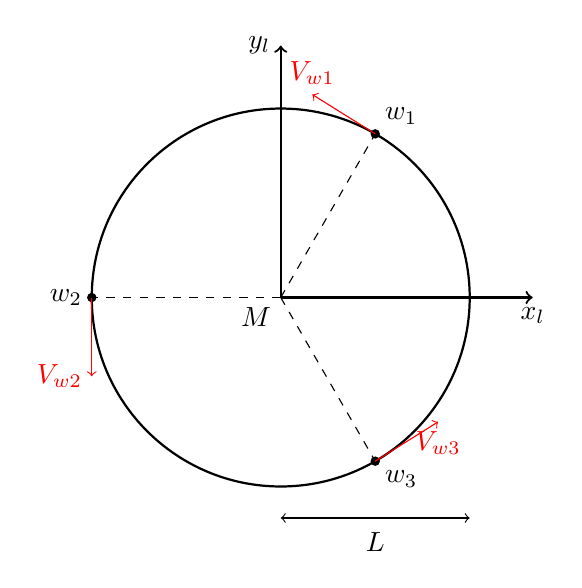
\begin{tikzpicture}[scale=2]

	% Mittelpunkt
	\coordinate (O) at (0,0);

	% Radius
	\def\L{1.2}

	% Radpositionen (deine Winkel)
	\coordinate (W1) at (60:\L);
	\coordinate (W2) at (180:\L);
	\coordinate (W3) at (300:\L);

	% Roboterkreis
	\draw[thick] (O) circle (\L);

	% Räder
	\fill (W1) circle (0.03) node[above right] {$w_1$};
	\fill (W2) circle (0.03) node[left] {$w_2$};
	\fill (W3) circle (0.03) node[below right] {$w_3$};

	% Radiuslinien
	\draw[dashed] (O) -- (W1);
	\draw[dashed] (O) -- (W2);
	\draw[dashed] (O) -- (W3);

	% Lokales Koordinatensystem
	\draw[->,thick] (O) -- (0,1.6) node[left] {$y_l$};
	\draw[->,thick] (O) -- (1.6,0) node[below] {$x_l$};

	% Geschwindigkeitsvektoren (tangential zu Kreis)
	\draw[->,red] (W1) -- ++(-0.4,0.25) node[above] {$V_{w1}$};
	\draw[->,red] (W2) -- ++(0,-0.5) node[left] {$V_{w2}$};
	\draw[->,red] (W3) -- ++(0.4,0.25) node[below] {$V_{w3}$};

	% Mittelpunktbeschriftung
	\node at (O) [below left] {$M$};

	% Radiusbeschriftung
	\draw[<->] (0,-1.4) -- (\L,-1.4);
	\node at (0.6,-1.55) {$L$};

	\end{tikzpicture}
	\caption{3-Rad-Omniroboter mit Radwinkeln $60^\circ$, $180^\circ$, $300^\circ$}
\end{figure}

Jedes Rad $w_j$ ist um einen Winkel $\alpha_j$ relativ zum Roboter-Koordinatensystem angeordnet.\\

Die Rollgeschwindigkeit $V_{wj}$ wirkt immer entlang der $y_{wj}$-Achse des jeweiligen Rades. Durch die freie Querbewegung entsteht zusätzlich eine seitliche (induzierte) $x_{wj}$-Komponente. Diese wird geometrisch aus der Projektion der anderen Räder berechnet. Betrachtet man beispielsweise Rad 1, so induzieren die Bewegungen von Rad 2 und Rad 3 eine seitliche Geschwindigkeit. Diese lässt sich durch Geometrische überlegung der Winkel und der Rollgeschwindigkeiten der anderen Räder bestimmen. Da die Räder im 120°-Winkel zueinander angeordnet sind, Tragen die anderen Räder mit einem Faktor von $cos(120^{\circ}-90^{\circ}) = cos(30^{\circ}) = \frac{\sqrt{3}}{2}$ zur seitlichen Geschwindigkeit bei, abhängig von der Richtung der Rollgeschwindigkeit.\\

Für Rad 1 ergibt sich also:
\[
V_{1,x1} = V_{w3}\cos(30^\circ) - V_{w2}\cos(30^\circ) = \frac{\sqrt{3}}{2}(V_{w3} - V_{w2})
\]

Die y-Komponente ist direkt:
\[
V_{1,y1} = V_{w1}
\]

Die resultierende Translationsgeschwindigkeit ergibt sich aus der Überlagerung aller Beiträge. Hierfür muss jedoch die Rotation in das Roboterkoordinatensystem berücksichtigt werden, da die Räder nicht entlang der Hauptachsen des Roboters angeordnet sind.

\begin{align}
\dot{x} &= \frac{1}{3} \sum_{j=1}^{3} V_{wj} \cdot (-\sin\alpha_j) \\
\dot{y} &= \frac{1}{3} \sum_{j=1}^{3} V_{wj} \cdot \cos\alpha_j
\end{align}
Die Rotationsgeschwindigkeit $\dot{\varphi}$ ergibt sich aus der Summe der Rollgeschwindigkeiten und dem Hebelarm $L$:
\begin{equation}
	\dot{\varphi} = \frac{1}{3L} \sum_{j=1}^{3} V_{wj}
\end{equation}

Damit ergibt sich allgemein:

\[
	\begin{bmatrix}
	\dot{x} \\
	\dot{y} \\
	\dot{\varphi}
	\end{bmatrix}
	=
	\begin{bmatrix}
	-\sin\alpha_1 & -\sin\alpha_2 & -\sin\alpha_3 \\
	\cos\alpha_1 & \cos\alpha_2 & \cos\alpha_3 \\
	\frac{1}{L} & \frac{1}{L} & \frac{1}{L}
	\end{bmatrix}
	\cdot \frac{1}{3}
	\begin{bmatrix}
	V_{w1} \\
	V_{w2} \\
	V_{w3}
	\end{bmatrix}
\]

Und konkret für den in diesen Projekt verwendeten Roboter für die Umrechnung der Motordaten in eine Bewegung in Roboterkoordinaten:

\begin{equation}
    \begin{bmatrix}
        v_x^{body} \\
        v_y^{body} \\
        \omega
    \end{bmatrix}
    =
    \begin{bmatrix}
        -\frac{\sqrt{3}}{3} & 0 & \frac{\sqrt{3}}{3} \\
		\frac{1}{3} & -\frac{2}{3} & \frac{1}{3} \\
		-\frac{1}{3R} & -\frac{1}{3R} & -\frac{1}{3R}
    \end{bmatrix}
    \begin{bmatrix}
        V_{\omega1} \\
        V_{\omega2} \\
        V_{\omega3}
    \end{bmatrix}
\end{equation}
Die Umrechnung Geschwindigkeit in Weltkoordinaten erfolgt dabei wiefolgt, wobei $\theta$ der aktuelle Winkel des Roboters im Raum ist:
\begin{equation}
    \begin{bmatrix}
        v_x^{world} \\
        v_y^{world}
    \end{bmatrix}
    =
    \begin{bmatrix}
        \cos(\theta) & -\sin(\theta) \\
        \sin(\theta) & \cos(\theta)
    \end{bmatrix}
    \begin{bmatrix}
        v_x^{body} \\
        v_y^{body}
    \end{bmatrix}
\end{equation}
Die Winkelgeschwindigkeit des Roboters ist in Roboterkoordinaten, als auch Weltkoordinaten gleich definiert, weshlab hier keine Unterscheidung vorgenommen wird.\\

Um schlussendlich die Position im Raum zu berechnen, integriert man die Geschwindigkeiten über die Zeit. Bei einer diskreten Integration mit einem Zeitschritt $\Delta t$ ergibt sich die folgende Formel für die Aktualisierung der Position:
\begin{equation}
    \mathbf{x}_{k+1} =
    \mathbf{x}_k +
    \Delta t \cdot
    \begin{bmatrix}
        v_x^{world} \\
        v_y^{world} \\
        \omega
    \end{bmatrix}
\end{equation}

% -------------------------------------------------------------------------------- %
% Beobachterstruktur
% -------------------------------------------------------------------------------- %
\section{Beobachterstruktur}
\begin{itemize}
    \item Luneburger
    \item EKF
    \item Zu beiden Blockschaltbilder erstellen
    \item Vergleichen und aufzeigen, warum EKF keinen bedeutenden Vorteil gegenüber Luneburger hat (Kamerafehler ist immer ähnlich, daher reicht statischer Gain)
\end{itemize}
\begin{figure}[H]
    \centering
    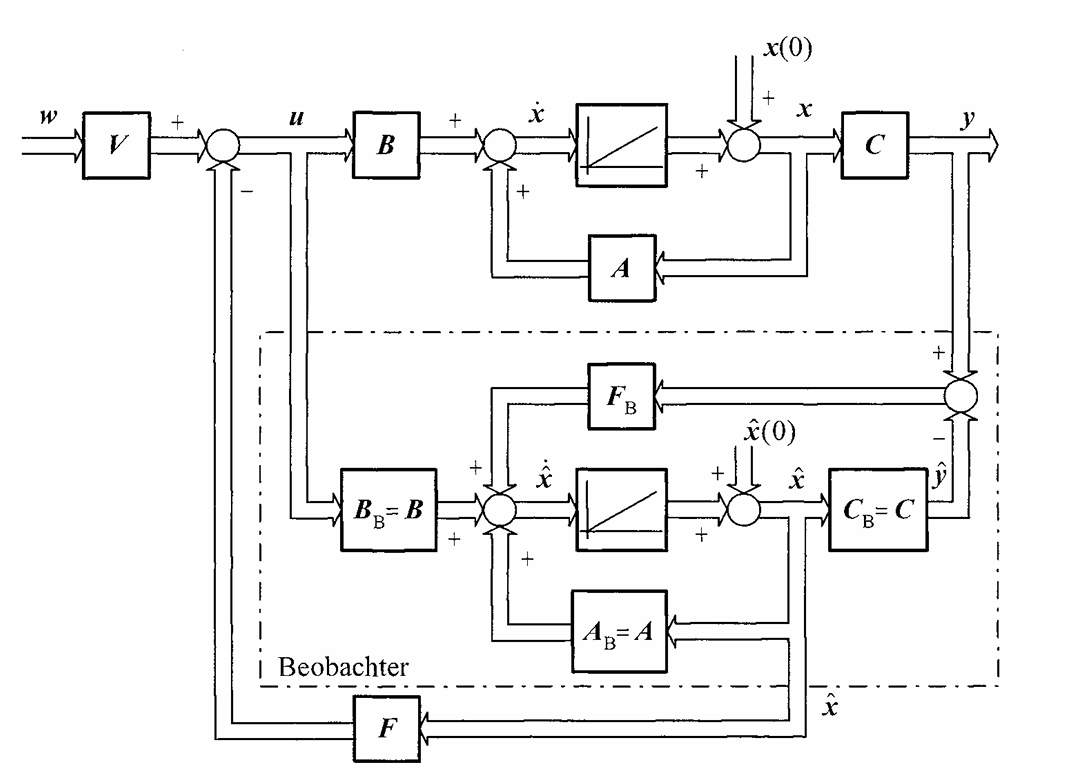
\includegraphics[width=0.8\textwidth]{_Bilder/LuneburgerBeobachter_Unbehauen.png}
    \caption{Zustandsbeobachter nach Luneburger \cite{lunze_regelungstechnik1}}
    \label{fig:LuneburgerBeobachter_Unbehauen}
\end{figure}

% -------------------------------------------------------------------------------- %
% Parametrierung/Auswertung
% -------------------------------------------------------------------------------- %
\section{Parametrierung/Auswertung}
\begin{itemize}
    \item Einstellen des Gains L
    \item Variabler Gain
\end{itemize}
\begin{figure}[H]
    \centering
    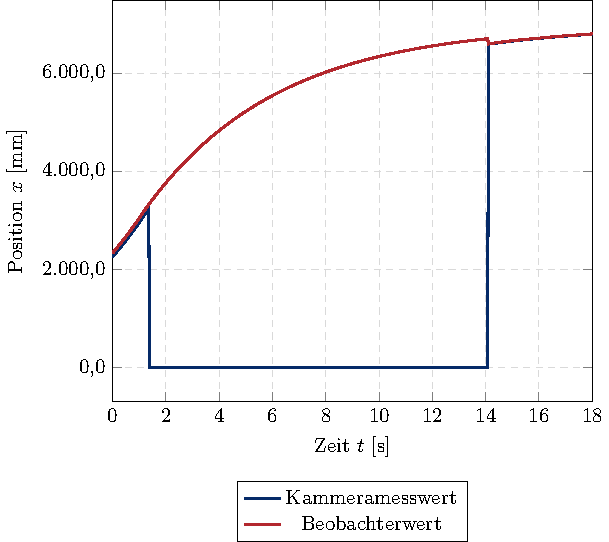
\includegraphics[width=0.8\textwidth]{_Grafiken/Obs_L1_Gesammt.pdf}
    \caption{Beobachter mit direktem Ausgleich Gesammt}
    \label{fig:Obs_L1_Gesammt}
\end{figure}
\begin{figure}[H]
    \centering
    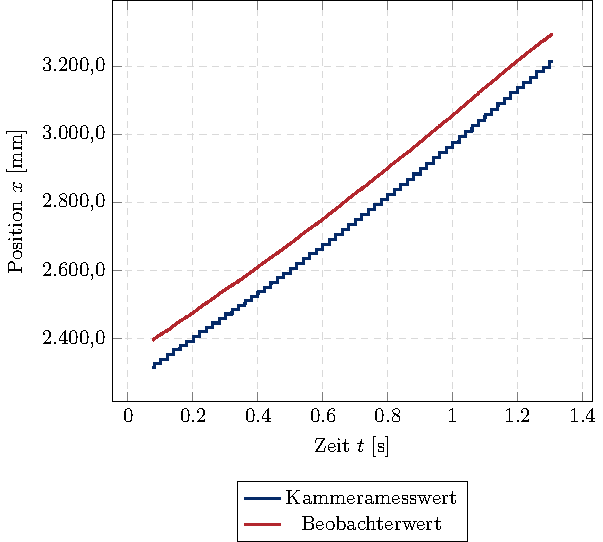
\includegraphics[width=0.8\textwidth]{_Grafiken/Obs_L1_Normalfahrt.pdf}
    \caption{Beobachter mit direktem Ausgleich Normalfahrt}
    \label{fig:Obs_L1_Normalfahrt}
\end{figure}
\begin{figure}[H]
    \centering
    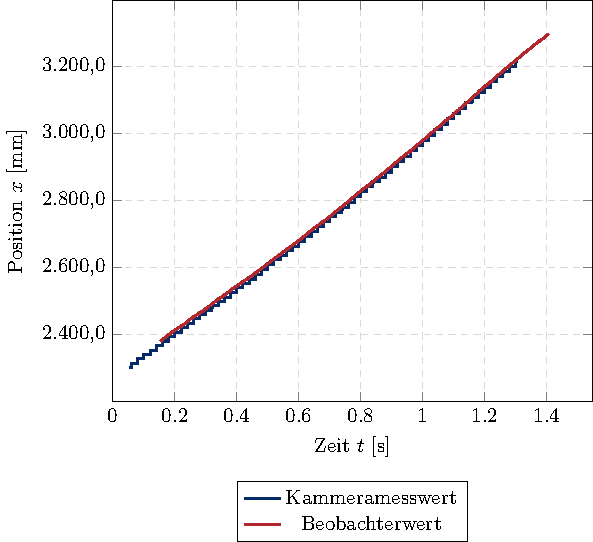
\includegraphics[width=0.8\textwidth]{_Grafiken/Obs_L1_NormalfahrtVerschoben.pdf}
    \caption{Beobachter mit direktem Ausgleich Normalfahrt Verschoben}
    \label{fig:Obs_L1_NormalfahrtVerschoben}
\end{figure}
\begin{figure}[H]
    \centering
    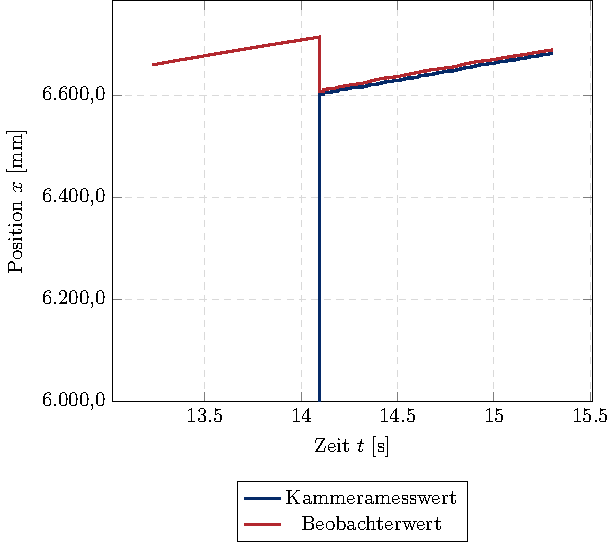
\includegraphics[width=0.8\textwidth]{_Grafiken/Obs_L1_Ausgleich.pdf}
    \caption{Beobachter mit direktem Ausgleich}
    \label{fig:Obs_L1_Ausgleich}
\end{figure}

\begin{figure}[H]
    \centering
    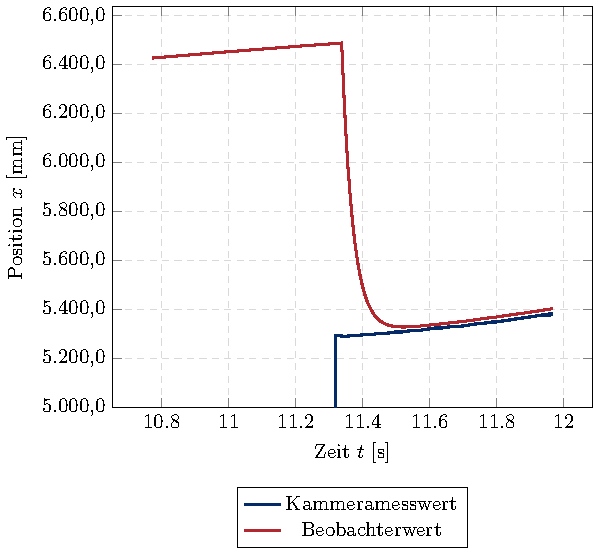
\includegraphics[width=0.8\textwidth]{_Grafiken/Obs_L01_Ausgleich.pdf}
    \caption{Beobachter mit langsamen Ausgleich}
    \label{fig:Obs_L01_Ausgleich}
\end{figure}

\begin{figure}[H]
    \centering
    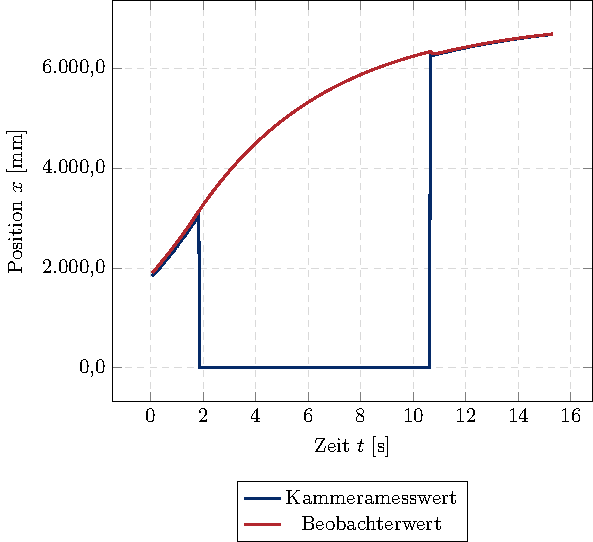
\includegraphics[width=0.8\textwidth]{_Grafiken/Obs_VarGain_Gesammt.pdf}
    \caption{Beobachter mit variablen Gain}
    \label{fig:Obs_VarGain_Gesammt}
\end{figure}
Is von der Idee her ganz nett, aber kein großer Effekt, da die Kamera, wenn Bild Erkannt, immer ähnlichen Fehler aufweißt. Also lieber statischen Wert tunen.